\section{Appendix B: Supplementary Forecasting Results}

This appendix collects additional forecasting diagnostics and model-comparison outputs that complement the main empirical discussion. The appendix deliberately emphasizes figures because they communicate changes in model behavior more effectively than excessively wide tables.

\subsection{Model-comparison figures}

\begin{figure}[H]
    \centering
    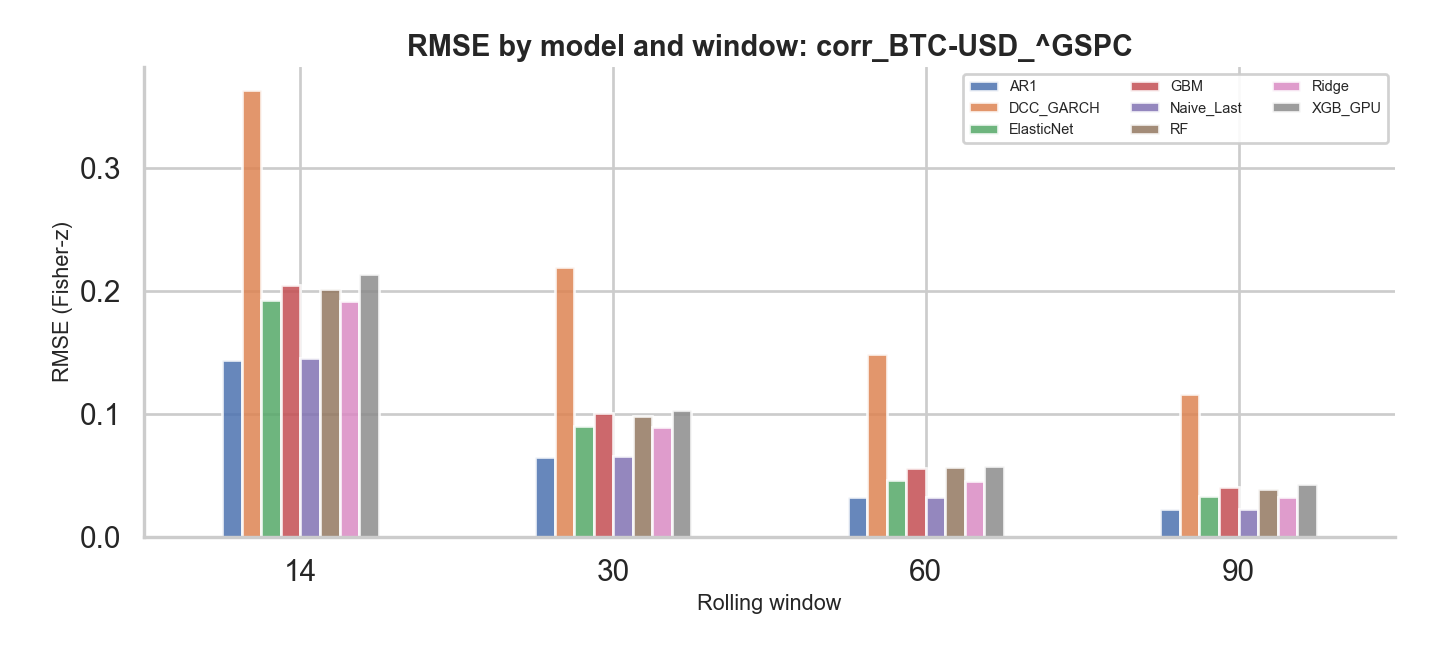
\includegraphics[width=0.8\textwidth]{../outputs/figures/model_rmse_comparison.png}
    \caption{Average RMSE comparison across model families.}
\end{figure}

\begin{figure}[H]
    \centering
    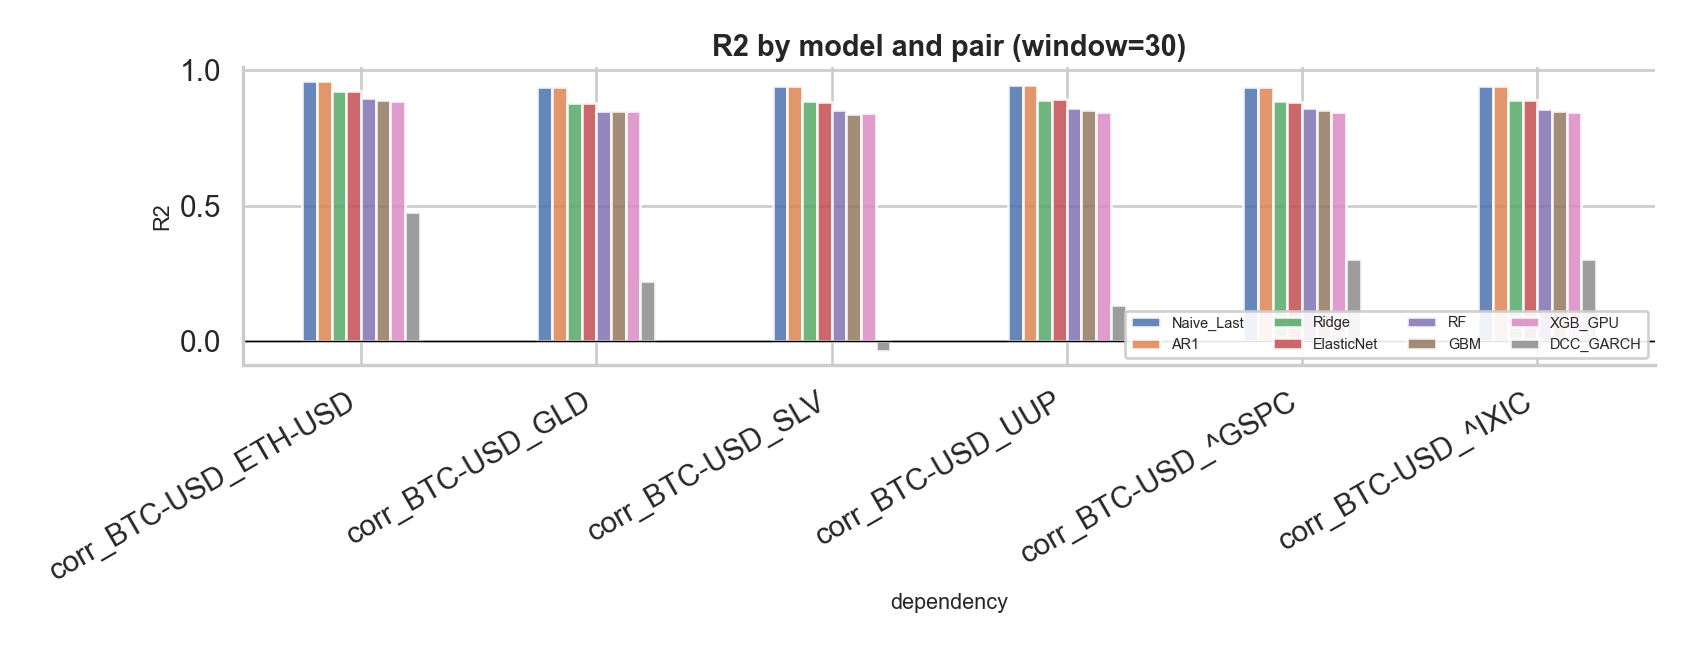
\includegraphics[width=0.8\textwidth]{../outputs/figures/model_r2_comparison_w30.png}
    \caption{Model $R^2$ comparison for the 30-day window.}
\end{figure}

\begin{figure}[H]
    \centering
    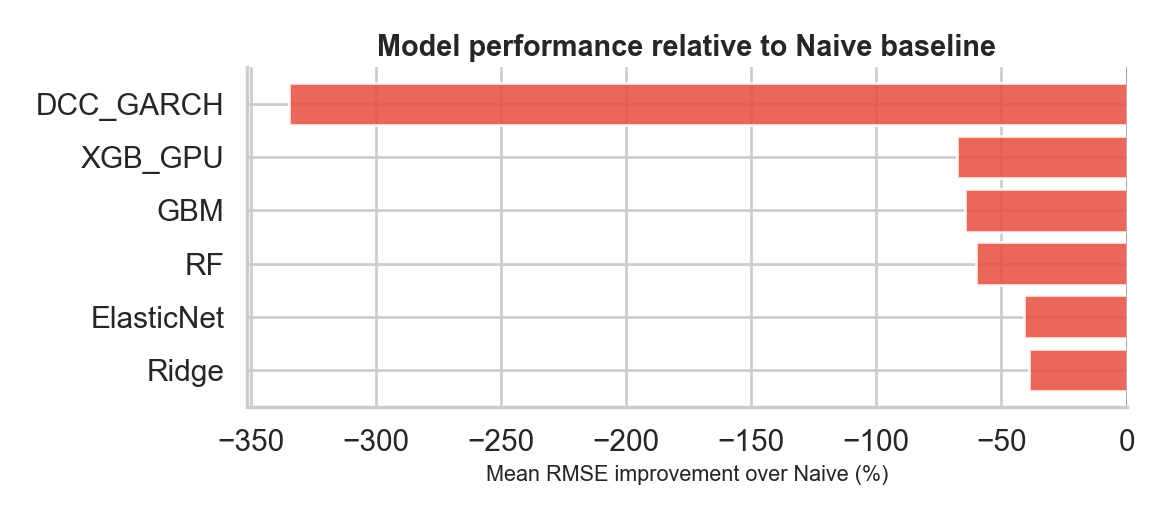
\includegraphics[width=0.8\textwidth]{../outputs/figures/model_improvement_over_naive.png}
    \caption{Improvement relative to the naive baseline.}
\end{figure}

\subsection{Hyperparameter and feature diagnostics}

\begin{figure}[H]
    \centering
    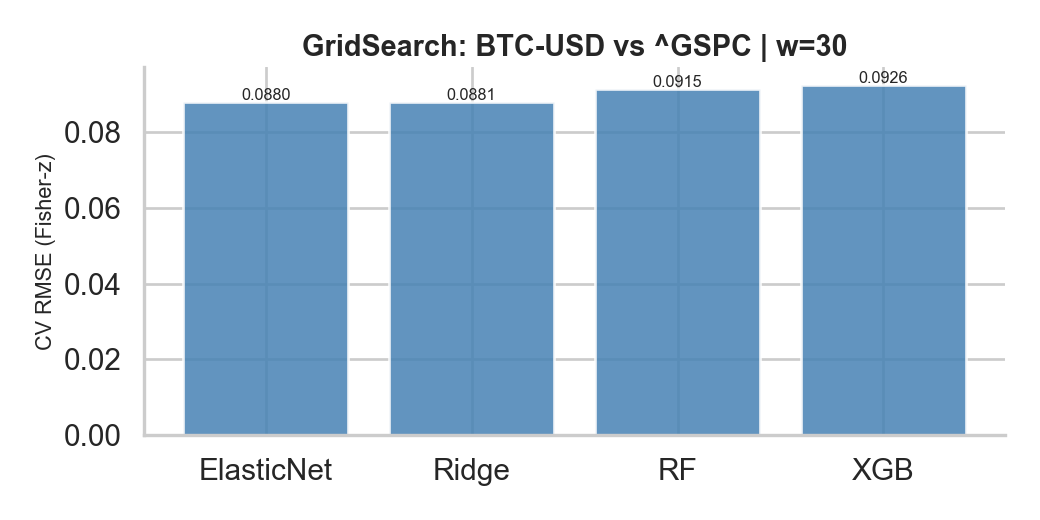
\includegraphics[width=0.8\textwidth]{../outputs/figures/gridsearch_cv_rmse_BTC-USD_^GSPC_w30.png}
    \caption{Grid-search cross-validation RMSE for the representative Bitcoin--S\&P 500 forecasting task.}
\end{figure}

\begin{figure}[H]
    \centering
    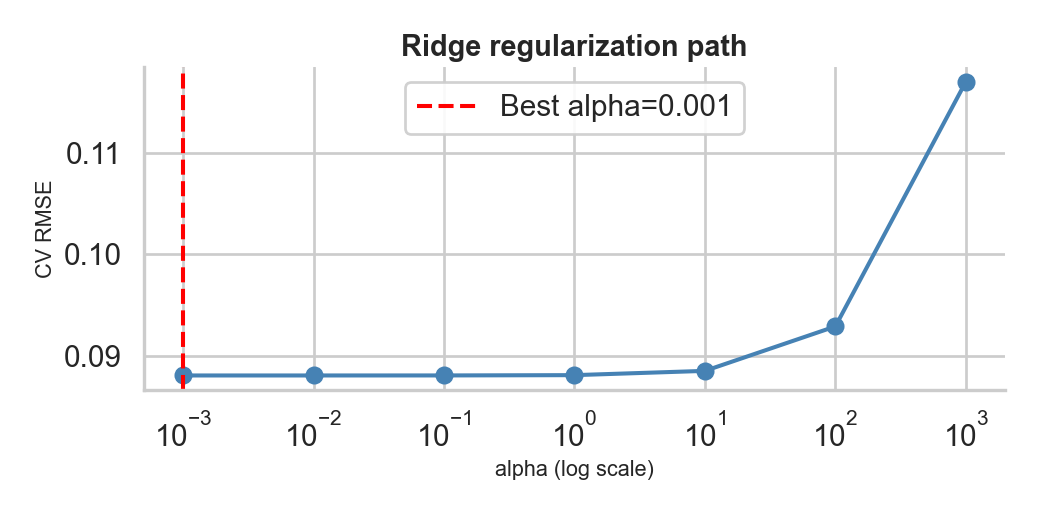
\includegraphics[width=0.8\textwidth]{../outputs/figures/ridge_regularization_path.png}
    \caption{Regularization path for the Ridge-based forecasting specification.}
\end{figure}

\begin{figure}[H]
    \centering
    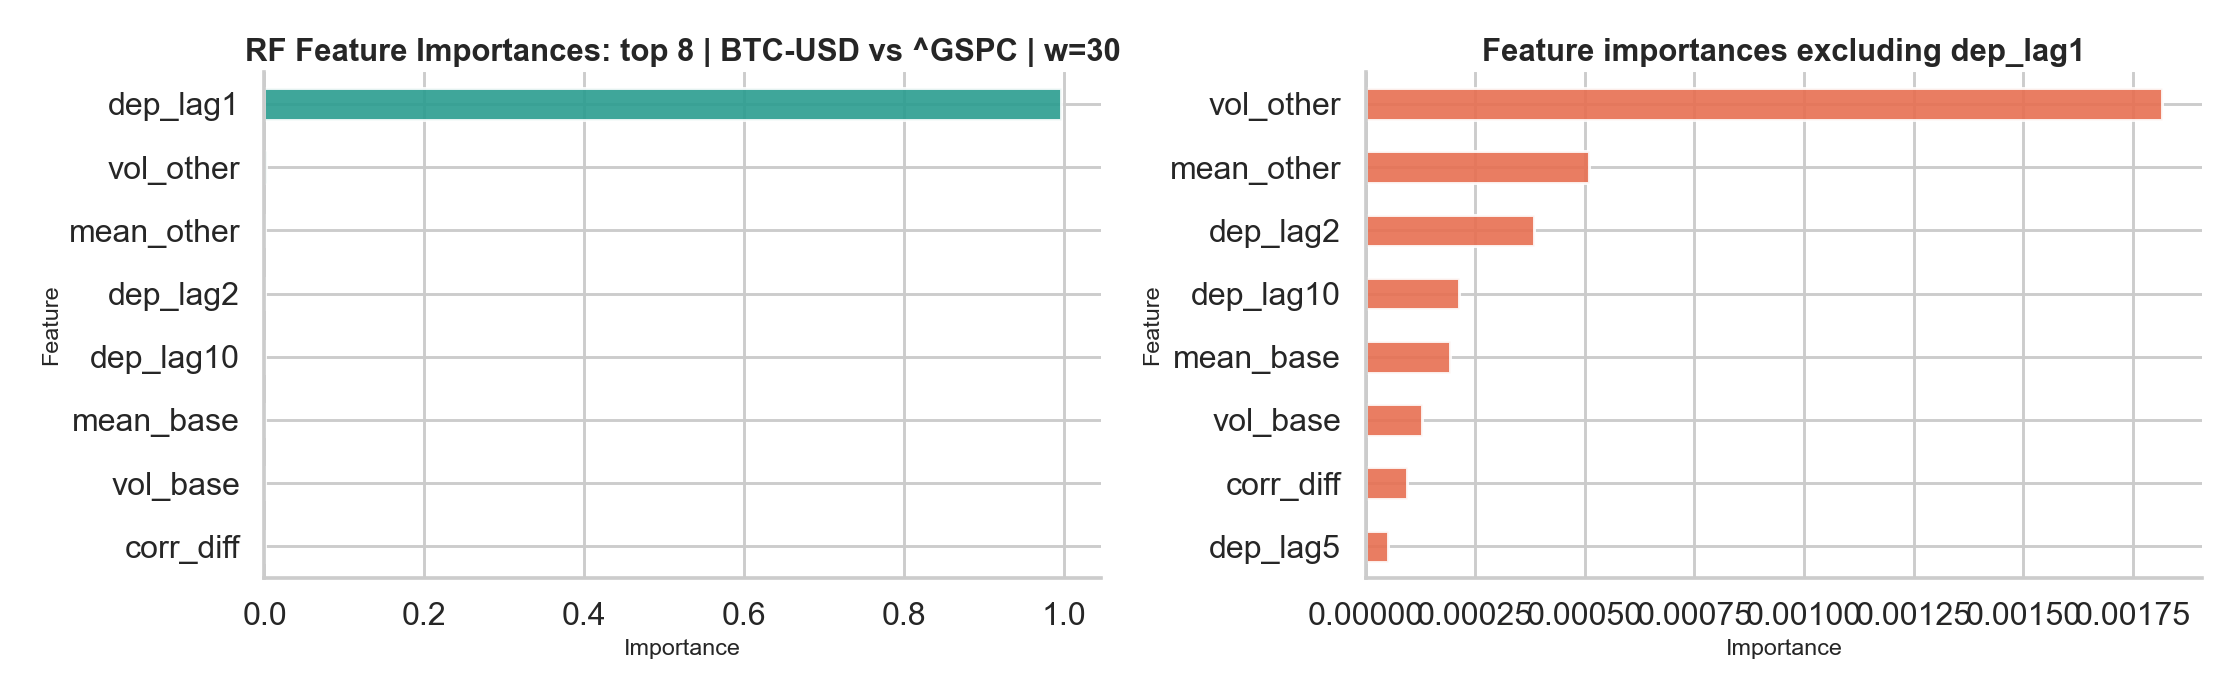
\includegraphics[width=0.85\textwidth]{../outputs/figures/rf_feature_importance_BTC-USD_^GSPC_w30_readable.png}
    \caption{Readable feature-importance view for the Random Forest model.}
\end{figure}

\subsection{Diagnostic plots for the representative equity pair}

\begin{figure}[H]
    \centering
    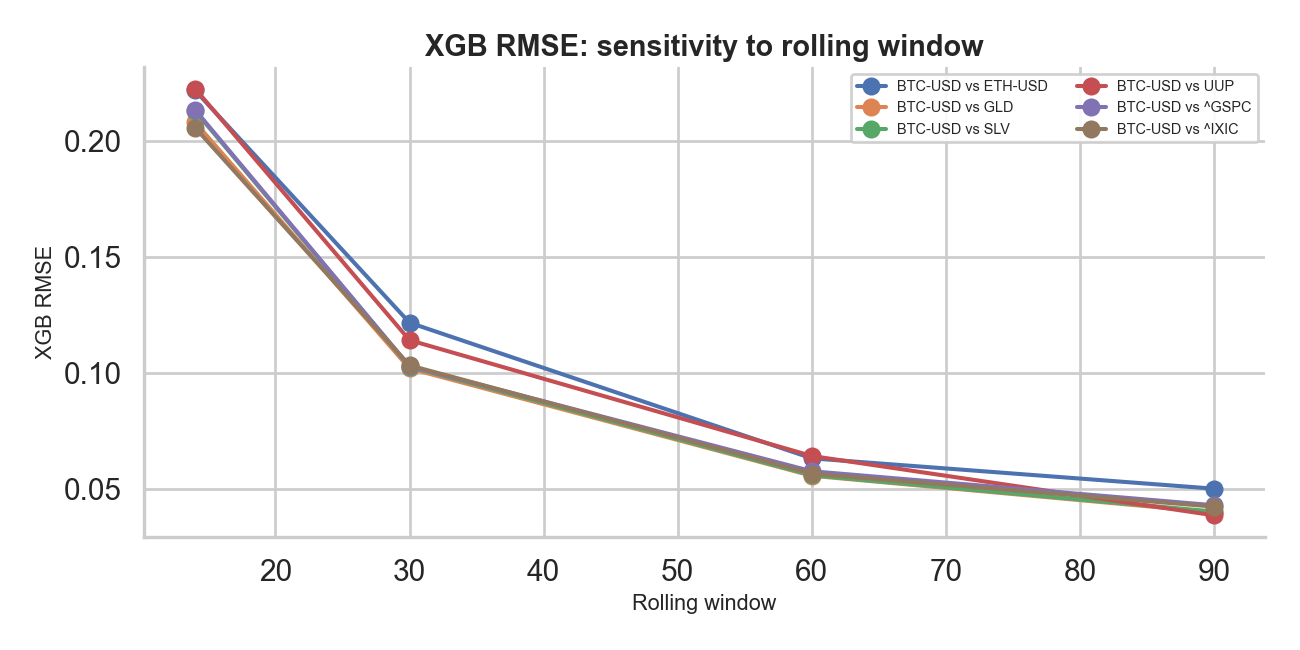
\includegraphics[width=0.82\textwidth]{../outputs/figures/xgb_window_sensitivity.png}
    \caption{Window sensitivity of the XGBoost-based forecasting layer.}
\end{figure}

\begin{figure}[H]
    \centering
    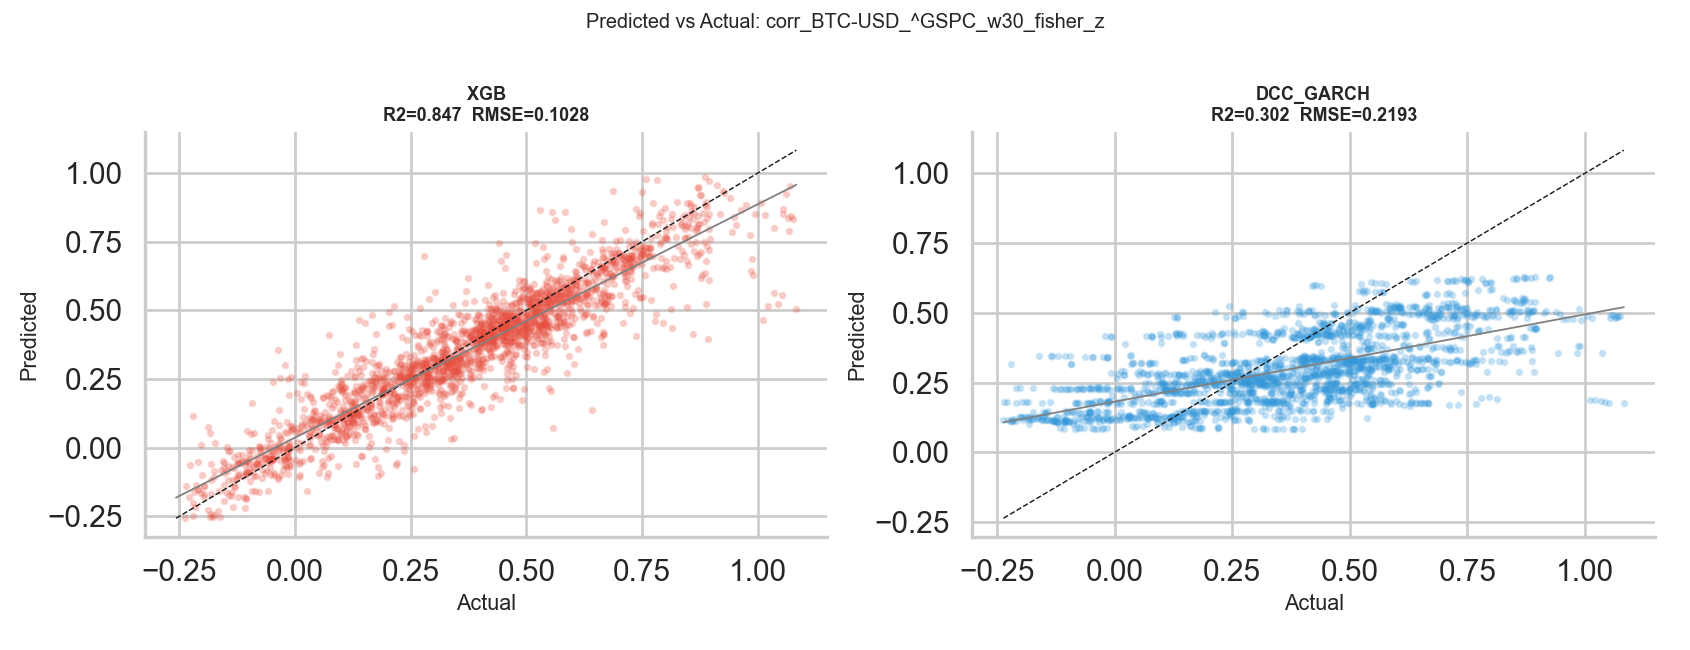
\includegraphics[width=0.82\textwidth]{../outputs/figures/scatter_corr_BTC-USD_^GSPC_w30_fisher_z.png}
    \caption{Forecast scatter diagnostic for the Bitcoin--S\&P 500 dependency experiment.}
\end{figure}

\begin{figure}[H]
    \centering
    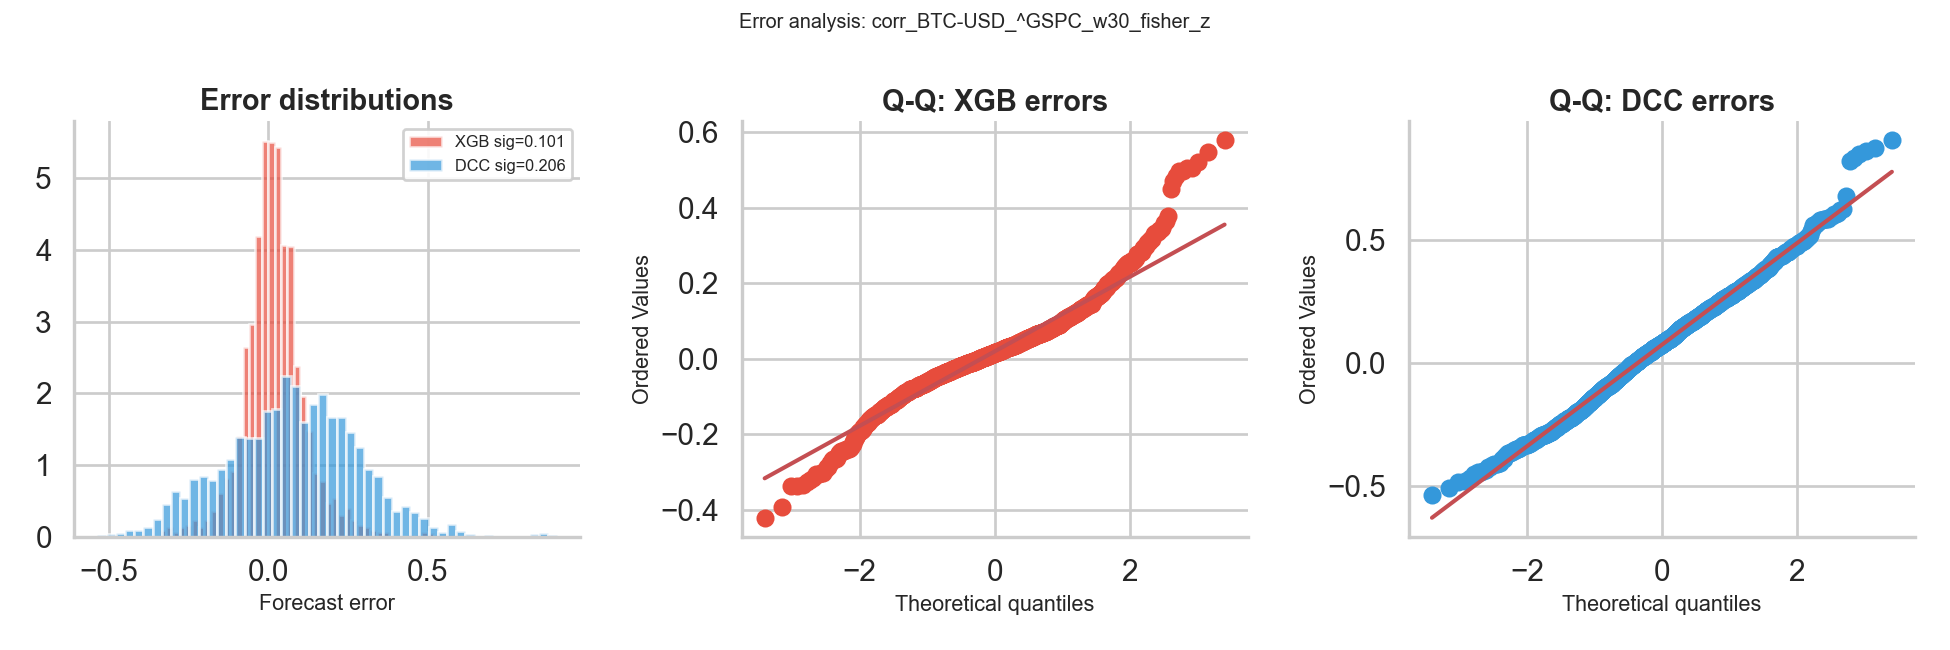
\includegraphics[width=0.82\textwidth]{../outputs/figures/error_dist_corr_BTC-USD_^GSPC_w30_fisher_z.png}
    \caption{Forecast error distribution for the representative Bitcoin--S\&P 500 dependency experiment.}
\end{figure}

\subsection{Sensitivity by asset pair}

\begin{figure}[H]
    \centering
    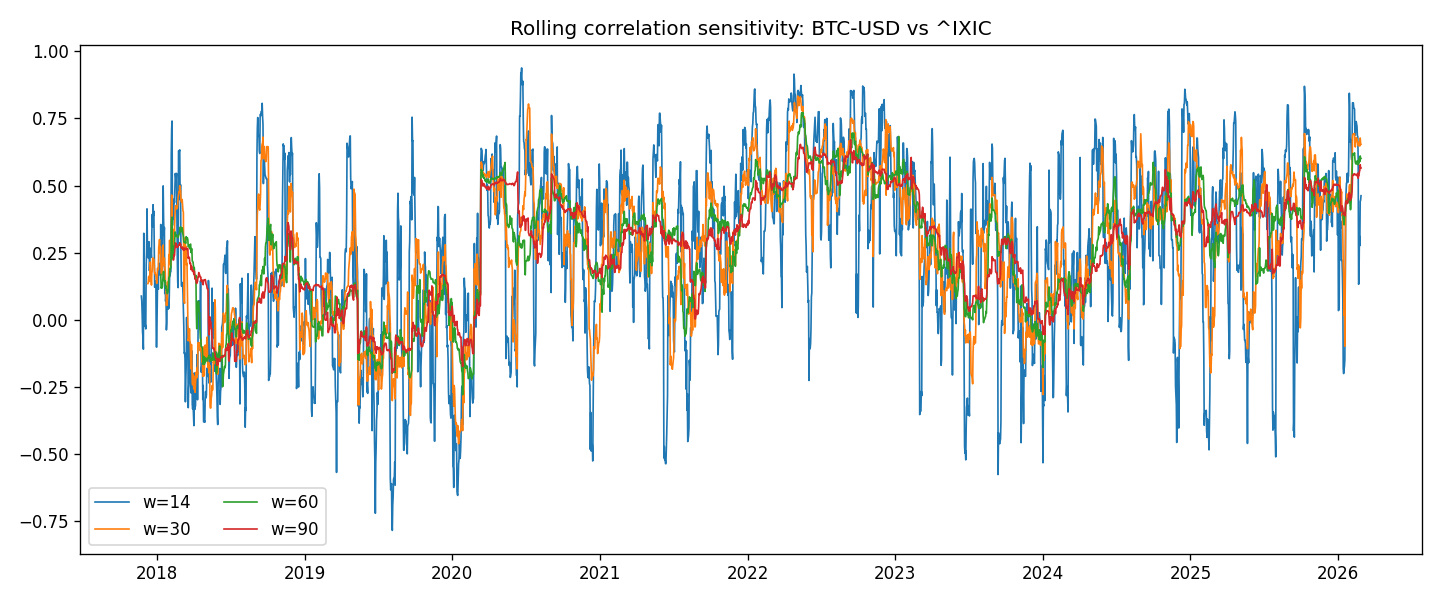
\includegraphics[width=0.9\textwidth]{../outputs/figures/sensitivity_BTC-USD_^IXIC.png}
    \caption{Sensitivity analysis for the Bitcoin--NASDAQ pair.}
\end{figure}

\begin{figure}[H]
    \centering
    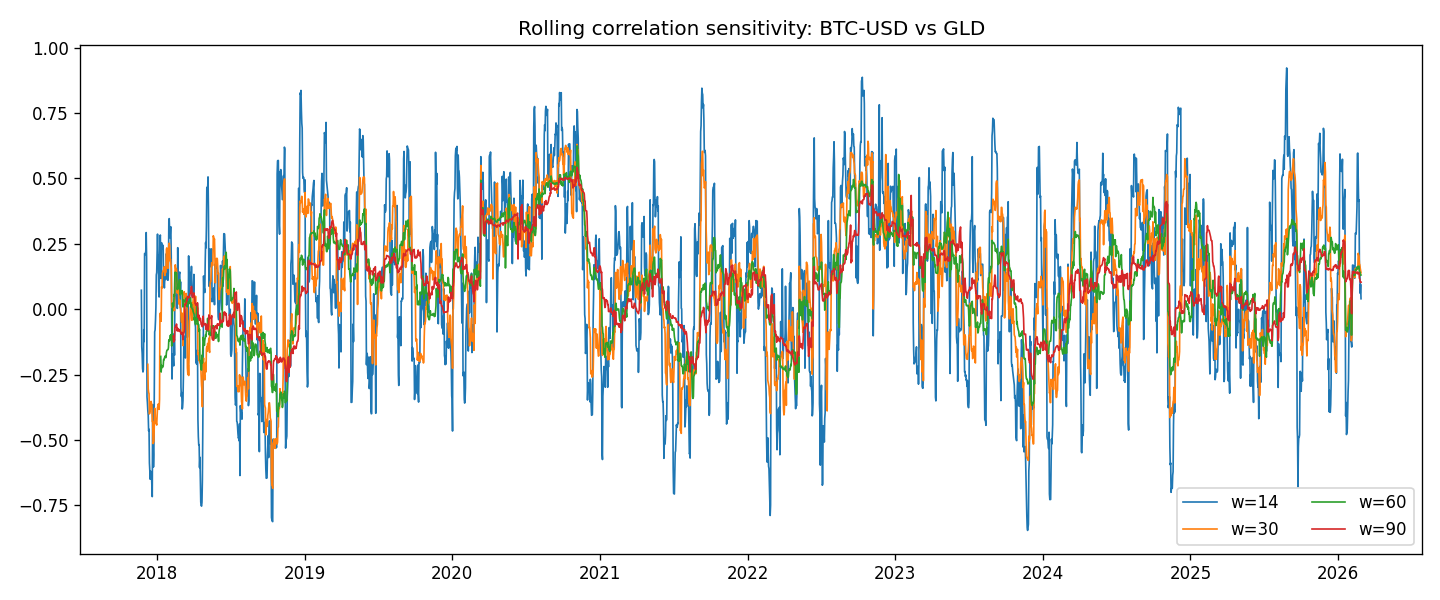
\includegraphics[width=0.9\textwidth]{../outputs/figures/sensitivity_BTC-USD_GLD.png}
    \caption{Sensitivity analysis for the Bitcoin--gold pair.}
\end{figure}

\begin{figure}[H]
    \centering
    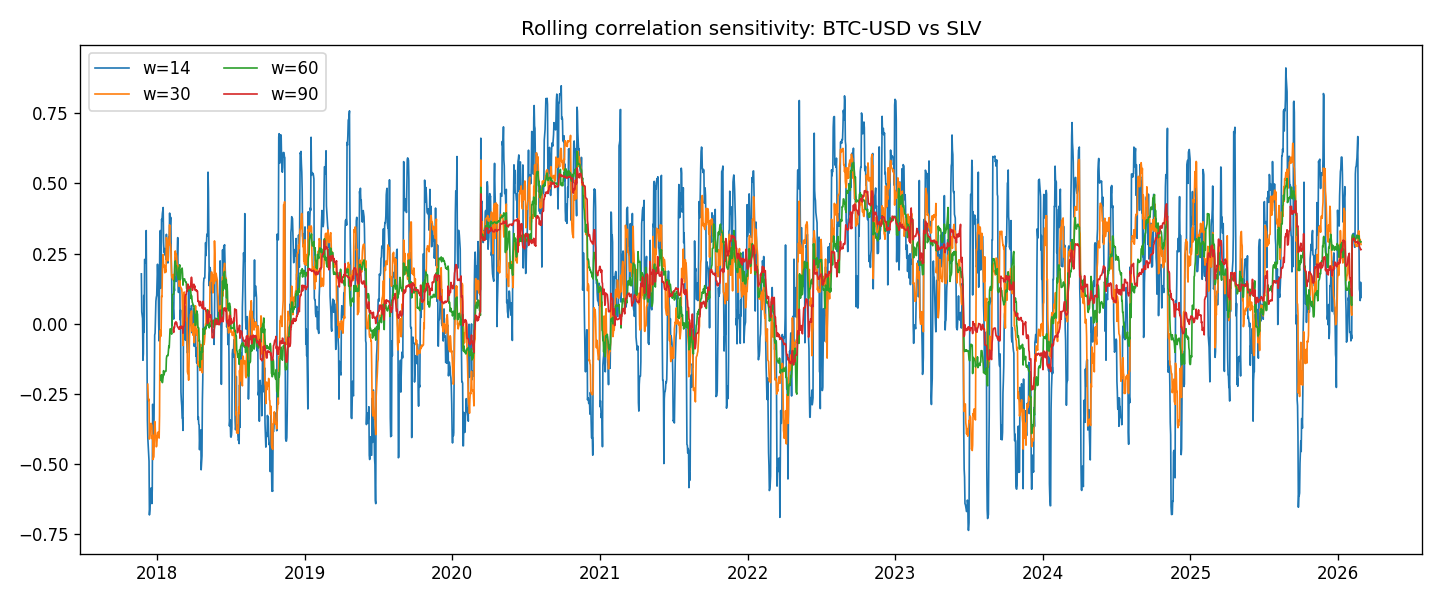
\includegraphics[width=0.9\textwidth]{../outputs/figures/sensitivity_BTC-USD_SLV.png}
    \caption{Sensitivity analysis for the Bitcoin--silver pair.}
\end{figure}

\begin{figure}[H]
    \centering
    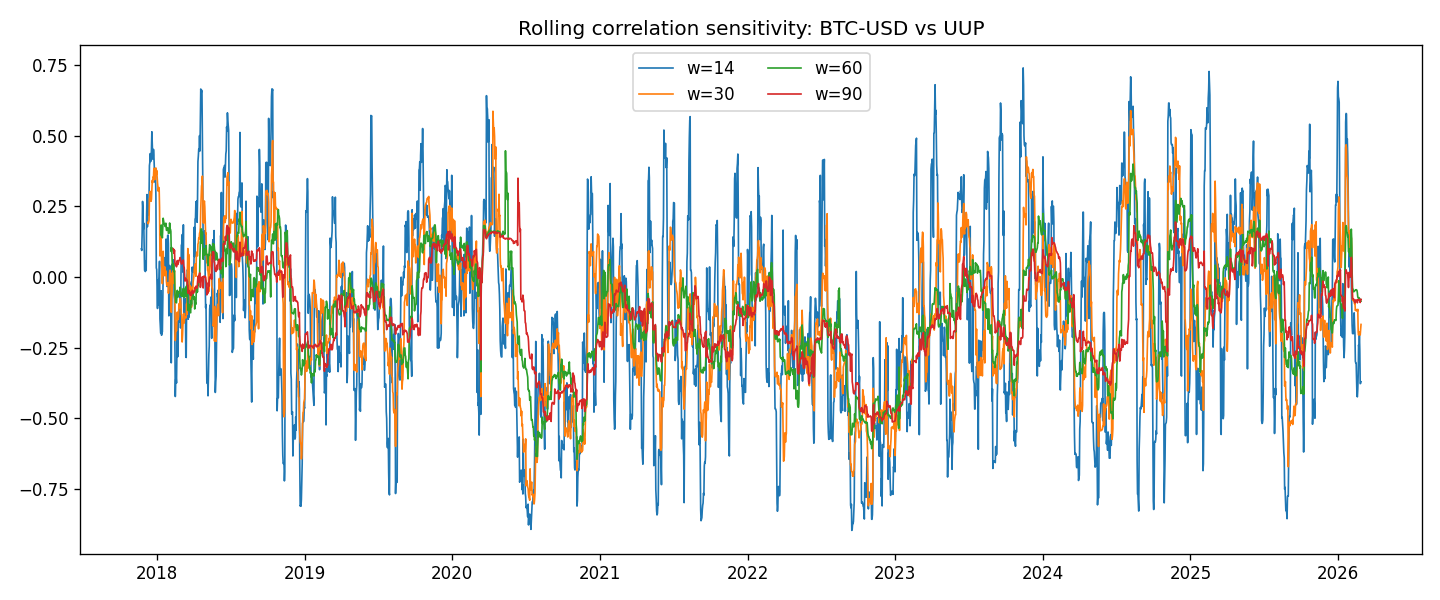
\includegraphics[width=0.9\textwidth]{../outputs/figures/sensitivity_BTC-USD_UUP.png}
    \caption{Sensitivity analysis for the Bitcoin--UUP pair.}
\end{figure}

\begin{figure}[H]
    \centering
    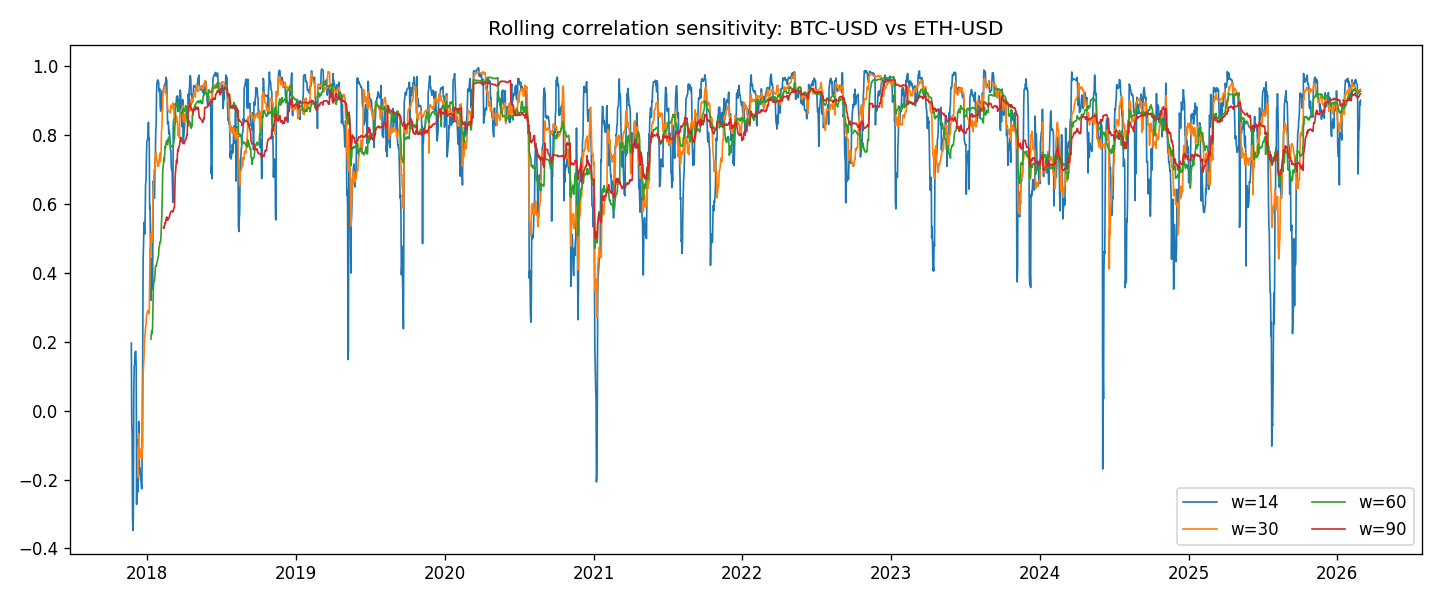
\includegraphics[width=0.9\textwidth]{../outputs/figures/sensitivity_BTC-USD_ETH-USD.png}
    \caption{Sensitivity analysis for the Bitcoin--Ethereum pair.}
\end{figure}

\subsection{Interpretation}

The supplementary figures reinforce several points made in the main text. Forecast quality depends materially on the choice of rolling window, the target remains strongly persistence-driven, and performance differences across model families are easier to interpret through comparative visuals than through a single ranking statistic alone.
